% TODO: tempted to term this "Module-aware dynamic fragmentation, analysis, and reassembly" as Dialysis or refracture
% CFP: https://www.usenix.org/conference/atc20/call-for-papers
\documentclass[letterpaper,twocolumn,10pt]{article}
\usepackage{usenix2019_v3}

\usepackage{soul}
\usepackage{xspace}
\usepackage{color}
\usepackage{booktabs}
\usepackage{graphicx}

\usepackage{caption}
\captionsetup[figure]{font=footnotesize,name={Fig.},labelfont={bf, footnotesize}}
\captionsetup[table]{font=footnotesize,name={Tab.},labelfont={bf, footnotesize}, skip=2pt, aboveskip=2pt}
\captionsetup{font=footnotesize,labelfont={bf, footnotesize}, belowskip=2pt}

\usepackage{enumitem}
\setlist{noitemsep,leftmargin=10pt,topsep=2pt,parsep=2pt,partopsep=2pt}

\def\omit#1{}
\def\eg{{\em e.g.}, }
\def\ie{{\em i.e.}, }
\def\etc{{\em etc.}\xspace}
\def\vs{{\em vs.}\xspace}
% \newcommand{\heading}[1]{\vspace{4pt}\noindent\textbf{#1}\enspace}
% No vspace, coz Usenix class already has paragraph space
\newcommand{\heading}[1]{\vspace{2pt}\noindent\textbf{#1}\enspace}
\newcommand{\ttt}[1]{\texttt{#1}}
\newcommand{\ttiny}[1]{\texttt{\footnotesize #1}}
\newcommand{\tcn}[1]{}

\definecolor{cdb}{rgb}{0.37, 0.62, 0.63} % cadet blue

\newcommand{\cf}[1]{(\emph{Cf}.\S\ref{#1})}
\newcommand{\sx}[1]{(\S\ref{#1})}
\newcommand{\tb}[1]{(Tab.\ref{tab:#1})}
\newcommand{\rf}[1]{\ref{#1}}
\newcommand{\se}[1]{\S\ref{#1}}
\newcommand{\fg}[1]{Fig.~\ref{#1}}

\newcommand{\sys}{{\scshape Lya}\xspace}
\newcommand{\toy}{{\tt lya.js}\xspace}


\newcommand{\fra}{fragmentation\xspace} % fracture
\newcommand{\ana}{analysis\xspace}      % 
\newcommand{\ass}{reassembly\xspace}    % 
\newcommand{\Fra}{Fragmentation\xspace} % fracture
\newcommand{\Ana}{Analysis\xspace}      % 
\newcommand{\Ass}{Reassembly\xspace}    % 
\newcommand{\dia}{\fra, \ana, and \ass}

% FIXME:
\newcommand{\pc}{PIC\xspace}
\newcommand{\pcs}{\pc{}s\xspace}

\newcommand{\goal}[1]{(\textbf{G#1})\xspace}

\newcommand{\nv}[1]{[{\color{cyan}#1 --- Nikos}]}
\newcommand{\review}[1]{{\color{red}#1}}
\newcommand{\TODO}[1]{\hl{\textbf{TODO:} #1}\xspace}
\newcommand{\todo}[1]{\hl{#1}\xspace}
\newcommand{\fixme}[1]{{\color{red}#1}}
\newcommand{\tc}{(\todo{cite})\xspace}
%-------------------------------------------------------------------------------
\begin{document}
%-------------------------------------------------------------------------------

%don't want date printed
\date{}

% make title bold and 14 pt font (Latex default is non-bold, 16 pt)
\title{\Large \bf Dynamic Program Dialysis with Lya}

%for single author (just remove % characters)
\author{
{\rm Anonymous Author(s)}\\
\normalsize{Submission \#225, 12 pages}\\
% \normalsize{Additional Anonymized Material: \href{https://git.io/JvfCf}{https://git.io/JvfCf}.}
% {\rm Grigoris Ntousakis}\\
% Technical University of Crete
% \and
% {\rm Nikos Vasilakis}\\
% Massachusetts Institute of Technology
}

\maketitle

\begin{abstract}

% Such library over-reliance is a recent trend: % in software engineering:
Applications today rely on hundreds of libraries, to the point where code written by their nominal developers is only a small fraction of their total line count.
% On the surface, such reliance is beneficial, 
Despite its benefits, this over-reliance creates many challenges, precisely due to the lack of knowledge of and visibility into library internals---for example, in the presence of deeply-nested third-party code, security auditing and performance profiling, already challenging in monolithic applications, become extremely difficult.

To address these challenges, we present \emph{program dialysis}, a novel dynamic-analysis technique specifically tailored to applications with many third-party libraries.
Combining name shadowing, context wrapping, and transformation of the underlying dependency graph, program dialysis automates dynamic \fra, \ana, and \ass of programs at the level of individual libraries during program execution.
% is a general technique that
It bolts onto existing languages, enabling analysis expressions in the source language, with only a few lines of analysis-specific code.
Our dialysis prototype, \sys, targets the JavaScript ecosystem counting over 1M libraries used on the web, server, and mobile.
We develop a series of case-studies to motivate \sys's design, and demonstrate how \sys allows the analysis of both individual libraries as well as multi-libraries application programs with low developer effort and performance overhead:
  insightful analyses can be expressed in 10--20 lines of code, add a virtually imperceptible increase in the load latency of individual libraries, and scale to real applications with hundreds of libraries.

% Module dialysis can be bolted on existing language runtime environments in a language-agnostic fashion 
% % By leveraging the ubiquity of third-party modules in today's applications
% Such modules can be part of third-party packages or of the language's standard library;
%   the latter is important for resources that are part of the broader environment where the application is executing, such as the operating system and the network.

% Operating at this level of granularity has several benefits:
%   (i) it allows bolting library dialysis itself as a library onto existing runtime environments that do not feature dynamic analysis,
%   (ii) it supports analysis expressions directly in the same language, tools, and abstractions as the host application language---eschewing low-level instrumentation, and %developers can use their tools 
%   (iii) it features low performance overheads, to the point that has the potential to be used online.
% % FIXME: It depends on the analysis
% % Due to the in the host language and at a coarser granularity than full-fledged dynamic analysis, module dialysis 
% % Operating at the granularity of library has several benefits: (i) ease (ii) performance (iii) while still getting 
% %In a sense, modules are the right level of abstraction 
\end{abstract}

\section{Introduction}
\label{intro}

Dynamic analysis is a type of program analysis performed by (and while) executing a program, with the goal of extracting information about the program and its execution.
Such information may include the ability to infer execution invariants, check security constraints, and extract performance characteristics~\cite{analysis:10}.
Contrary to other types of analysis, its key benefits make it the primary (or only) candidate in a variety of scenarios---namely, ones that require:
  (i) current runtime information, such as profiling information, in view of changing load patterns~\cite{staticdynamic},
  (ii) accurate visibility into the execution, devoid of abstraction or approximation~\cite{staticdynamic},
  (iii) Turing-complete policies, where policies themselves are programs~\cite{contracts1, contracts2, contracts3},
  (iv) dynamic or runtime-reflection features, such as the ones present in Python and JavaScript~\cite{jsanalysis1, jsanalysis2}.

% Where dynamic analysis shines is
% Dynamic analysis occupies a clear spot in the space of analysis has clear strengths and weaknesses.
% Examples of information not analyzable statically include runtime code evaluation, runtime introspection and reflection, as well as multi-lingual support.
% Dynamic analysis is a particularly good fit for the analysis of dynamic languages.

Unfortunately, reaping these benefits comes with significant costs in terms of developer effort or runtime performance.
Manually instrumenting a program requires a good understanding of its internals. % instruction sets?
External tools such as instrumentation frameworks~\cite{pin, valgrind} and performance tracing tools~\cite{perf, dtrace} only add to the curve, as they feature their own language for specifying analyses. % usually different from the application's language.
Modifying the application's runtime environment such as the interpreter is cumbersome, error-prone, and requires development in a language that is different than that of the program.
Tools that virtualize execution~\cite{pin, valgrind, jalangi, roadrunner} have high performance costs---for example, Jalangi~\cite{jalangi} and RoadRunner~\cite{roadrunner} report No-Op analysis on the order of 26--32$\times$ and 52$\times$, respectively.
% Problem-specific solutions require significant investment outside the language's mental model---for example,  each ---as a case in point, Jalangi reports XX overhed (exact overheads always depend on the specific analysis).

Effort and performance costs are severely compounded by the use of third-party libraries, usually glued together without a full understanding of their internals.
This is a recent phenomenon enabled by zero-cost code sharing~\cite{libs}:
% Libraries are used pervasively today to lower development costs and improve software quality, 
% This over-reliance to third-party libraries is a recent phenomenon, 
  language-specific package repositories eliminate the cost of publishing and using a library.
As a result, applications frequently count hundreds of libraries~\cite{npmstudy:19}, with each often only a few lines long~\cite{leftpad, npmstudy:19}. % how to say thousands of them depend on a 11-line lib?
Library-oriented analysis adds to the challenges of prior tools as
  (i) library boundaries disappear at runtime, and
  (ii) coarse-grained, high-level language semantics misalign with fine-grained, low-level instrumentation.

To address these challenges, we propose a novel approach to dynamic analysis, termed \emph{dialysis}\footnote{
  A method of deconstruction into elements often for the purposes of removing waste products or altering piecewise components.
  From ancient Greek {\scriptsize $\delta\iota\acute{\alpha}$} (di\'{a}, ``inter-, through'') and {\scriptsize $\lambda\acute{\tilde{\upsilon}}\epsilon\iota\nu$} (lúein, ``to loosen'').
} and implemented in \sys.
Program dialysis is a general technique, applicable to any programming language, that enables dynamic fragmentation, analysis, and re-assembly of applications at the level of individual libraries. 
It operates during program execution, automating wrapping and transformation of the program's dependency graph, and allowing developers to extract meaningful insights with only a few lines of analysis-specific code
By operating at the granularity of libraries, dialysis has several benefits over prior work: %full-fledged dynamic analysis:
  (i) it allows bolting library dialysis itself as a library onto existing runtime environments with no dynamic analysis,
  (ii) it supports analysis expressions using the same language, tools, and abstractions as the host program language,
  (iii) it features significantly low runtime performance overheads, enabling the potential for toggling its use in production environments.

% (i) at a somewhat coarser granularity, but still offering insights---and in a semantics-aware way tailored to the programming language.
% (ii) bolt on
% Our approach is applicable to any language that supports some notion of modularity, runtime introspection, and .
% It plugs into the module-loading capability of the runtime system to insert key hooks for inserting 
% After the parsing and interpretation phases of module loading complete, 
%  which are then parsed and interpreted and 
% Surprisingly, as we show in this paper, this architecture requires \emph{no} modifications to the language runtime---that is, it is backward-compatible with vanilla unmodified language runtime environments.
% 
% Its key strategy is to fracture applications at the boundaries of modules, instrument their interfaces (including direct accesses) using meta-programming capabilities, and recombine them 
% By combining visiiblity into both built-in and third-party modules, \sys can get gather important information for 
% at a much lower cost---both in terms of runtime performance and developer effort.
% 
% % to enable module-aware dynamic analysis are general
% To achieve this, module-aware dynamic analysis leverages several techniques.
% It plugs into the module manager;
% wraps interfaces
% (i) bolt on, meaning
% (ii) high-performance, and 
% (iii) low effort 
% 
% As shown later, these capabilities are generally available in all dynamic programming languages---\eg 

To demonstrate its effectiveness, we evaluate \sys on the JavaScript ecosystem (>1.2M libraries~\cite{modulecounts}). % and unusually high code-reuse~\cite{npmstudy:19}. %, and a pressing need for usable dynamic analysis~\cite{}.
We develop a diverse set of analyses that target practical information about a program:
  an allow/deny security analysis,
  a profiling analysis showing bottlenecked modules,
  a synthesis-oriented analysis on input-output data, and
  an analysis enforcing a static union-based type system at runtime.
This set of analyses drives the design requirements for \sys, and highlights dialysis as a middle ground between coarse- and fine-grained analysis.
We evaluate \sys at three different levels:
  (i) synthetic micro-benchmarks that test certain aspects and confirm the correctness of our analyses in a controlled environment;
  (ii) single-module meso-benchmarks that allow comparison with dynamic analysis frameworks; and
  (iii) end-to-end full-application macro-benchmarks that show behavior of \sys on realistic workloads. 
\S\ref{bg}--\ref{eval} present our key contributions:
\begin{itemize}
\item \S\ref{bg} characterizes the shared needs of four case-study multi-module analyses whose needs remain mostly unmet by general-purpose analysis frameworks.
\item \S\ref{design} presents the design of the bolt-on module-oriented dynamic analysis~\sx{design}, which meets the requirements of the four case-study analyses.
\item \S\ref{impl} discusses our implementation, \sys, as a pluggable library for the JavaScript ecosystem, as well as the implementation of the four analyses.
\item \S\ref{eval} evaluates \sys showing it expresses insightful analyses succinctly, adds minimal overheads over the baseline runtime, and scales to hundreds of modules.
\end{itemize}

Aside from the aforementioned sections (\S\ref{bg}--\ref{impl}), the paper discusses \sys's limitations and its application to other languages~\sx{diss};
  it compares with related prior work in the literature~\sx{rw};
  and closes with appropriate conclusions~\sx{end}.


\section{Background, Examples, and Goals}
\label{bg}

A single application today often incorporates multiple libraries written and published by several different authors.
To make the difficulties of analyzing such library-overreliant more concrete, we describe several example analysis that are often needed by the authors of third-party libraries.
These examples illustrate key requirements for the design of a framework for analyzing applications at the boundaries of modules.
Before describing these examples, however, we offer a brief refresher on the abstractions and corresponding internals of module systems~\sx{bg1}.

% The emerging development process should (and to a certain extent, does) simplify the development and testing process;
%   unfortunately, good abstractions are sealed (\ie they do not leak between abstraction layers), which makes the inspection of a library difficult.

\subsection{Background on Module Systems}
\label{bg1}

A library, package, or module---we use these terms interchangeably---is a development-time construct for encapsulating reusable functionality.
This functionality falls into two categories:
  it either (i) comes bundled with the language, possibly wrapping operating-system interfaces such as the file-system in a way that is system-agnostic and conforms to the language's conventions,
  or (ii) is provided by other developers sharing code others might find useful.
Fig.~\ref{mod} depicts the basic structure of a modern program, in which the \ttt{math} library provides a set of four elementary operations.

From a developer's perspective, \ttt{import}ing a library makes its functionality usable by the calling code. 
What this means is that some of the library's functionality is bound to a variable name that becomes available in the scope of the caller.
This is provided through a form of \ttt{export}ing, where the library developer expresses which values should become available to the importing code.
The definition of a value depends on the semantics of the language, but for now we can assume it's either a primitive value, a list of values, a function, or an object mapping string keys to values.
Internally, the library might import other libraries, cause side-effects to the file-system and the network, or even be implemented in multiple languages.
% , as shown on line \fixme{XX},
% closely coupled with the runtime
% and in some cases features its own mini-language, as is the case in Scheme and Standard ML.

From the language's perspective, the loading process is achieved in several steps. 
In compiled programming languages libraries might be used to enable separate compilation, in which case an additional linking phase connects the resulting object files.
Interpreted languages involve a somewhat convoluted process that combines loading, interpretation, and linking.
This process starts by locating the library in the file system or across the network,\footnote{
  Examples of run-time environments featuring network loading include V8 and deno, for executing JavaScript and TypeScript respectively.
}
by resolving relative or absolute identifiers.
% The library is assigned a unique identifier.
The content of the library is then read and wrapped in a way that resolves library-local names such as \ttt{\_\_name\_\_} in Python and \ttt{\_\_filename} in JavaScript to meaningful values.
The wrapper is then interpreted and evaluated using the language's interpreter, which might result to side-effects---for example, a \ttt{process.exit} in the library's top-level scope will exit the entire program.
Finally, the value returned bound to the \ttt{export}ed interface or returned from this interpretation (depending on the language) will be made available to the scope of code calling \ttt{import}.

There is significant variation, but a few features are common across many implementations.
A library cache maintains a mapping from library identifiers---often absolute paths---to returned \ttt{export} values.
The library cache serves a dual purpose:
  by avoiding to locate already loaded libraries, it improves performance and maintains the consistency of stateful libraries.
Recursive imports are handled in depth-first way, and if cyclical dependencies are possible they are resolved by pointing to the cache.
An increasingly common feature is to allow different versions of the same library to co-exist in a program, in order to avoid a choice between mutually exclusive options---a paradoxical situation known as ``dependency hell''.
As a result, a single \ttt{import} \ttt{lib} does not necessarily resolve to the same (version of the) library \ttt{lib} every time.
The dual of this situation is also possible, in which two different library names may resolve to the same identifier (in which case the second will be redirected to the cache).
These features complicate library-level analysis, especially in interpreted programming languages.


% Several details:
%   same module at multiple levels, and the module cache
%   sometime it's the same, some times it;s not
%   module resolution algorithm

\subsection{Motivating Examples}

Having reviewed the building blocks and underlying techniques that power modularity, we now turn to examples of dynamic analysis that today are difficult or require specialized solutions:
  (i) an allow/deny security analysis,
  (ii) a profiling analysis showing hot libraries,
  (iii) a synthesis-oriented analysis on input-output data, and
  (iv) an analysis enforcing a static union-based type system at runtime.
These examples illuminate key design requirements for \sys's implementation of module-level dynamic analysis.

\heading{Security Analysis}
The pervasive reliance on third-party libraries has led to an explosion of supply-chain attacks~\cite{long2015owasp, maass2016theory, snyk, lauinger2017thou}.
Both bugs and malicious code in imported libraries create attack vectors, exploitable long after libraries reach their end-users.
As library boundaries do not exist at runtime, libraries end up executing with no meaningful isolation or privilege separation guarantees between each other and the trusted portions of a program.
Popular libraries, depended upon by tens of thousands of other libraries or applications, allow vulnerabilities deep in the dependency graph to affect a great number of applications~\cite{leftpad, npmstudy:19}.
Discovered vulnerabilities are becoming harder to eradicate, as updates are fetched automatically~\cite{npmFailure} and module unpublishing is becoming a multi-step process to avoid breaking applications~\cite{npmUnpublish}.
Worst of all, leaked publishing tokens allow attackers to update packages with code that will eventually reach end-users via package updates~\cite{eslint1}.

As a concrete example, consider the recent event-stream incident~\cite{es1, es2}, in which a maintainer of a highly popular library inserted code for stealing Bitcoin wallet credentials from a program using that library.
As event-stream activated its malicious behavior only on production---\ie not during testing or development---it is critical to be able to toggle the behavior of the system
At the same time, it is not critical to analyze behavior \emph{within} the event-stream library itself:
  if any data exfiltration is happening, this will require calling out of the library and into the network---in event-stream's case, using the \ttt{fs} library to modify a different library and then use \ttt{http} from the second library.
Both \ttt{fs} and \ttt{http} are libraries part of the standard library and built into the runtime environment.
% The key issue underlying the \ttt{event-stream} attack is that any third-party fragment of an application has unrestricted access to the functionality available to the rest of application.

To address such problems, several recent proposals suggest analyzing third-party modules dynamically to identify malicious behavior~\cite{}.
% FIXME more about the policy, tracking arguments too
A simple ``allow-deny'' security analysis indicating the resources touched by that library would have revealed access to the and access .
Examples of interfaces outside the \ttt{http} and \ttt{fs} libraries include the ability to use global variables, import other libraries, and access the cache of the loaded modules---all of which are easily available to any third-party that is part of an application.

% \emph{
% This case highlights the need to \fixme{analyze} all the observable behavior \emph{around} a library, without necessarily caring about fine-grained library-internal analysis.
% }

\heading{Performance Diagnosis}
Diagnosing performance problems is a difficult task, exacerbated by the heavy use of third-party libraries.
Libraries are written by authors with different education backgrounds, quality standards, and, most importantly, needs:
  it's not unusual for a weekend project solving a local need to end up as a critical dependency among several open source projects~\cite{}.
Maintenance and rewriting can cause performance regressions between two versions of a library.
% FIXME: Garbage collection
Worse even, the fact that one library changes a dependency to a different implementation can cause severe performance pathologies to upstream projects---that is, while the interface remains the same due to an intermediate layer of abstraction, performance characteristics change dramatically~\cite{evhaus}.

As a concrete example, consider the \ttt{minimatch} library, a regular-expression-based file-matching utility susceptible to long delays because of pathological regular expressions that involve backtracking.
Pathological inputs reaching \ttt{minimatch}, even if benign, can cause significant performance degradation.
The source of this degradation can lie deep in the dependency chain of the application~\cite{crosby2003denial}, but also affect logically unrelated parts competing for the same resource (\ie CPU).

The research community has proposed several possible mitigations~\cite{}, all critically depending on detecting and attributing the slowdown to the bottlenecked component.
An analysis 
% A key observation is the semantic isomorphism between calling a function and passing a message
% This allows viewing a series of calls as a stream of messages.
% Module boundaries can be viewed as (virtual) queues of messages that await processing.
treating library invocation boundaries as message queues~\cite{scheme:98, duality:79}.
Overwhelming a module causes its ingress queue to grow.
At some point, the waiting time of newly-arrived messages becomes longer than sending messages to a library replica.
Profiling is accomplished by wrapping module interfaces with logic that generates a model of the current workload.
Each module boundary collects its own statistics based on a combination of recipes and instructions from the coordinator.
Profile generation can operate at a high resolution in time and space:
  (i) at every function call entering a module, and (ii) on thousands of modules across an application.


% ATTRIBUTION
% Interestingly, profiling functions running at each boundary cannot ``see through'' libraries in order to attribute load among a library and its dependencies correctly.
% For example, an agent at the outermost boundary \ttt{A} of a dependency tree \ttt{A}$\rightarrow$\ttt{B}$\rightarrow$\ttt{C} does not know how much of the latency\eat{ is \ttt{A}-internal and how much} comes from \ttt{B}. % or \ttt{B}'s dependency, \ttt{C}.
% 

% \emph{
% This case highlights the need to \fixme{analyze} all the observable behavior \emph{around} a library, without necessarily caring about fine-grained library-internal analysis.
% }

\heading{Invariant Discovery}
Extracting type invariants is helpful in a variety of ways---type safety is an important property and types are lightweight annotations that can be quickly and efficiently checked.
Dynamic analysis can be used to generate type assertions or invariants
For example
e.
For example, types identify program invariants to be preserved during code modifications, to generate marshalling and marshalling wrappers, or even to guide library synthesis and regeneration.
This is especially problematic in dynamic programming languages:
  in the absence of type signatures, there is not much one can say about a \ttt{http.request} object.

To make this concrete, consider the case of the \ttt{gRPC} library for serializing and de-serializing objects.
Given a ---say, a simple bignum library or a crypto---a developer has to first run the library manually, take note of the result, and then write a protocol buffer specification file declaring the type; %, common in distributed systems
if the type changes, because of a library version change or because of changes in the .

The static type system is defined as a variant of a simply-typed lambda calculus augmented with union types.
A simple approach would be to define a very simple type system that captures the type of a value by observing the execution of the program---after all, the types are dynamically checked!
The analysis could also capture union types, for cases where it observes that a variable is at times witnessed to hold values of different types---although a single program tends to make calls of the same type signature across its entire lifetime~\cite{daikon}.
The analysis could also do some type ``unpacking'' to deconstruct a type to its structural primitives---for example, noting that an object of type user is comprised of two strings (first and last name) and a number (age).

% would need to be able 
% to capture structural subtitling---that is the piecewise 


% \heading{Learning, Synthesis, and Regeneration}

\subsection{Design Goals}

We have briefly introduced four motivating analyses for extracting information about an application's dependencies.
While the challenges behind these analyses share several characteristics, today they remain largely unaddressed by dynamic analyses frameworks due to a combination of factors:
  these frameworks either require highly specialized solutions often outside the core language,
  do not leverage or offer semantic information at the level of module boundaries, or
  lead to a high (often impractical) performance overheads due to the high granularity of their analyses.
To summarize, these applications would appear to be served well by a system that:
\begin{itemize}
  \item \textbf{(G1)} Operates at the level of modules, leveraging both the semantics and performance potential that this level of granularity potentially offers.
  \item \textbf{(G2)} Does not require learning a new tool or language, but rather allows developers to express their analyses on the same language as the program.
  \item \textbf{(G3)} Can be implemented as a library that bolts onto an existing language runtime environment.
\end{itemize}

The next section describes program dialysis, a new program analysis technique that satisfies these goals, in a language-agnostic manner~\sx{design};
  the section following that describes a concrete implementation for the server-side JavaScript ecosystem~\sx{impl}.

\section{The Design of Program Dialysis}
\label{design}

Dialysis starts by dynamically modifying the functionality of the module system that is responsible for importing and loading libraries:
  instead of simply locating and loading a library from the file-system, it yields control to \sys, which applies a series of transformations to libraries with the goal of interposing at their boundaries.
We start with an overview of dialysis~\sx{overview}, highlighting several key challenges, followed by a detailed description of each step~(\S\ref{one}--\ref{three}).

\subsection{Overview}
\label{overview}

% FIXME: add user data
At a high level, the goal of program dialysis is to dismantle the program at the boundaries of third-party libraries, apply transformations that insert analysis-specific machinery, and then carefully assemble individual components to maintain the original semantics.
 In more detail:

\begin{itemize}
  
  \item \textbf{Dismantling:}
Dialysis starts by recursively dismantling a program into its dependencies. % ---pieces of software implement a computation or functionality.
This is achieved by re-wiring the language's \ttt{import} functionality to go through \sys, resulting in \sys walking the program's recursive dependency structure at runtime.
During this phase, \sys has to determine the granularity of the analysis (\eg top-level libraries, a specific library \etc) in order to apply transformations at the correct level and mapping provided analysis hooks to the corresponding libraries.

  \item \textbf{Transformation:}
It then sets up the provided analysis, by transforming each library interface, its surrounding environment, and possibly the values passing through the library boundary.
Programmatic transformations walk and wrap each one of these values based on their type.
% the library interface is usually a complex (but singular) object;
% the surrounding environment provides names to multiple ``implicitely'' imported libraries, functionality provided by the language.
This phase requires solving several challenges, including enumerating all points of entry into and exit out of a library, 
and swapping original values externally available to a library with ones that are wrapped with interposition mechanisms.

  \item \textbf{Re-assembly}
Finally, dialysis re-assembles individual modified libraries back into the program's original structure.
The most important challenge during this phase the treatment of the library cache~\sx{bg1}:
  since a single library can now correspond to many different wrappers, each modified to capture a small fragment of the overall analysis, the cache needs to be augmented to ensure the right analysis fragment clicks at the right place during the re-assembly of the dependency tree.

\end{itemize}

% Program runtime transformations such as the ones applied in the second phase are used pervasively throughout \sys.

\begin{figure}[t]
\raggedleft 
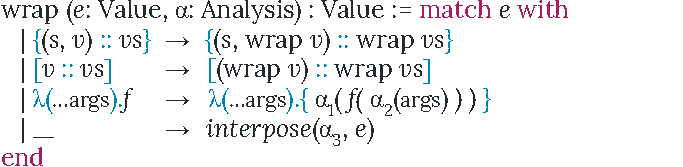
\includegraphics[width=0.45\textwidth]{./figs/lya_base.pdf}
\caption{
  \textbf{Base transformation.}
  \textmd{
  The algorithm (simplified) is presented in functional style to simplify variable binding; types (object, list, function, and primitive), used for pattern matching, are shown in light {\color{cdb} \emph{turquoise}}~\cf{bt}. The meta-function $\alpha$ stands for the locations of analysis hooks.
  }
}
\label{fig:base}
\end{figure}

% To transform a module, \sys augments several steps of the module loading process (Fig.~\ref{fig:pipeline}) using a base transformation that wraps an object with a security monitor~\sx{bt}.
% It starts by intercepting calls to the \ttt{require} function~\sx{import}, which locates the module's source code and \pc.
% It then constructs a custom context based on the \pc's implicit segment~\sx{context}.
% It then encloses the module in a closure to leverage local variable resolution in order to link the custom context with the module~\sx{enclosure}.
% After source interpretation, \sys transforms the resulting value by consulting the \pc's explicit segment~\sx{final}, updates the \sys-augmented module cache~\sx{cache}, and returns the value to the consumer.
% The following subsections detail these steps.

\subsection{Dismantling}
\label{one}

When the dialysis starts along with the rest of the program, it first loads the analysis hooks provided by the developer. 
Among other things, \sys needs to determine which library boundaries are of interest and what the granularity of the analysis is going to be.
For the former, developers may have specified a subset of libraries whose boundaries are of interest or a subset of libraries that should \emph{not} be analyzed.
For the latter, it checks the constructs that---for example, whether the analysis includes global variables, library-local constructs, standard libraries \etc

It then dynamically replaces the implementation of\ttt{import}:
  rather than simply locating and loading a library, the function yields to \sys.

\sys checks the cache~\sx{three} to determine (i) if the library has already been loaded, and (ii) whether it has been loaded with the same analysis hooks.
If both are determined true, \sys retrieves the cached version of the library and returns the transformed \ttt{export}ed value.
If the library was loaded with a different analysis---say because there are different analyses applied to different parts of a dependency tree---\sys constructs the appropriate analysis and applies a transformation pass on a cached copy of the unmodified library~\sx{three}.
% \omit{---the common case---}
Otherwise, \sys first invokes the built-in library loader to locate the library.

The process of loading new libraries includes (i) a phase of reading the necessary files as source code and (ii) a phase of interpreting them, interspersed by applications of transformations.
Reading files returns a string representation of the code; interpretation uses the language's runtime evaluation primitives to convert the code to an in-memory object.
A series of transformations is applied before and after interpretation~\sx{two}.

Some analyses may themselves make use of global variables, libraries, and other analyzable constructs.
\sys must note not to include these constructs in the ones 
% The analysis language is embedded in the source language, thus \sys makes use of the language's built-in evaluation primitives to interpret the \pc specification file.
Dialysis frameworks may want to add analysis-specific keywords not provided by the language.
To achieve this, \fixme{we} wrap each analysis hook with a function whose body starts by defining the expected keywords.
The precise techniques for achieving this will be made clear in the next section~\sx{two}, after covering transformations;
  the key to remember is that analysis are loaded from disk as source files, similar to libraries.

\begin{figure}[t]
\centering 
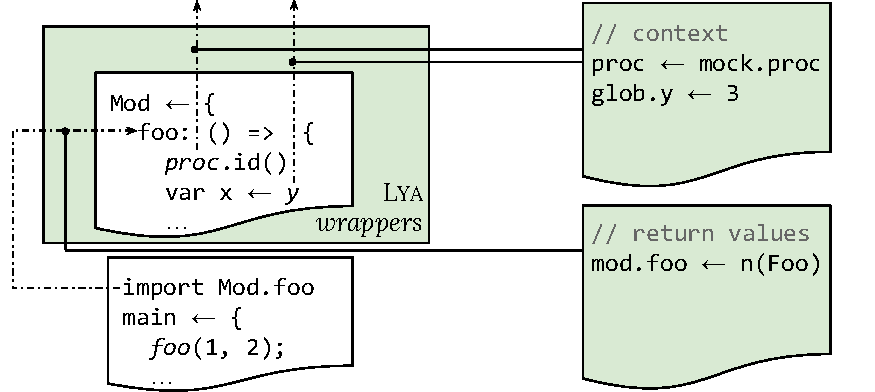
\includegraphics[width=0.45\textwidth]{./figs/lya_shadowing.pdf}
\caption{
  \textbf{Shadowing segments.}
  \textmd{
  Cross-module variable name resolution (left) augmented with \sys (green boxes), which interjects non-bypassable steps resolving to \sys-augmented values (right-top: implicit module imports; right-bottom: explicit import).
  }
  \vspace{-4mm}
}
\label{fig:shadowing}
\end{figure}


\subsection{Transformation}
\label{two}

For each analyzed library, \sys needs to place hooks all around its boundary---not just its interface.
This is achieved in three logical steps:
(i) transforming the variable context, a mapping from names to values, within which the library will be interpreted,
(ii) interpreting the library within this context, so that all names resolve to \sys-augmented values, and
(iii) transforming the return value, \ie the library interface, once the interpretation is complete.
Before discussing \emph{where} each transformation are applied, however, it makes sense to see \emph{how} they are applied.

\heading{Transformations}
% , such as an object returned from a module or an exception about to be sent across the network.
Transformations can be applied to any value in the language, which can generally be a primitive, a function, or a compound value---say, a list of values or an object of key-value pairs.
% Listing~\ref{core-tx} presents a simplified core of the language.
Transformations walk compound values from their root, processing component values based on their types (Fig.~\ref{fig:base}).
More specifically,
  (i) \emph{function} values are wrapped by closures that contain analysis-specific hooks; % on the function's arguments and return values;
  (ii) \emph{object} and \emph{list} values are recursively transformed, with their getter and setter methods replaced similar to function values; % and at times combining return results; and
  (iii) \emph{primitive} values are either transformed directly or copied unmodified and wrapped with an access interposition mechanism.
To avoid cycles during the walk, values are added to map that is consulted at the beginning of each recursive call.
% Usually transformations do not mutate original values, but first copy them, apply transformations to the copies, and return copies to the caller.


% \sys's transformations boil down to a base form \ttt{BT} that augments \emph{objects} with runtime security monitors.
% At a high level, \ttt{BT} takes an object $O$ and a \pc $\sigma$ and returns a new object $O'$.
% Every field $f$ of $O$ is wrapped with a method $f'$ defined to enclose $f$.
% At runtime, $f'$ checks $\sigma$:
%  if the access is allowed, it forwards the call to $f$;
%  otherwise, it raises an exception.
% % Appendix: An example result is shown in the appendix.~\ref{fig:bt2}.
% 
% To achieve this transformation, \sys walks the object graph from the root and processes component values based on their types (Fig.~\ref{fig:base}).
% Rather than mutating original values, it copies them, applies transformations on the copies, and returns copies to the caller:
% 
% % Listing~\ref{core-tx} presents a simplified core of the language.
% 
% \begin{itemize}
% \item
%   \emph{function} values are wrapped by a closure that forwards arguments to the original function if allowed to do so.
% \item
%   \emph{object} values are recursively transformed, with their getter and setter methods replaced similar to function values.
% \item
%   \emph{primitive} values are copied unmodified and wrapped with an access interposition mechanism.
% \end{itemize}

Direct field accesses, such as assignments, require custom detection upon dereference.
To achieve this, \sys wraps fields with an interposition mechanism;
  this mechanism essentially treats direct field accesses as function calls (see \S\ref{impl} for implementation details and \S\ref{reqs} for equivalents in other environments).
% Examples of such mechanisms include \ttt{Proxy} objects (JavaScript), metatables (Lua), metaclasses (Python), and direct-accessor metaprogramming (Ruby).
\sys's wrappers detect and record changes to any of the object's fields, transforming values as needed.
For example, if a field in a transformed object is assigned a new value, that value itself has to be be transformed before being attached to the \fixme{tree}.

\sys allows toggling analyses on/off, changing analysis, or chaining multiple analysis during the execution of the program.
To achieve this, it maintains a handle to the root of both the unprocessed and the newly processed values, for further processing:
  the unprocessed value is used to create objects, at runtime, that run a different analysis;
  the new value is used to revoke or chain analyses, a feature not explored further in this paper.

\heading{Context Transformation}
To be able to track an analysis at the library boundary, \sys needs to provide each library with values that are augmented with interposition wrappers---and do this for all of the names a library to which a library has access.

To achieve this, \sys first needs to prepare a transformed copy of the library's outer context.
Semantically, the context is a map from variable names to their values.
Thus, \sys creates an auxiliary hash table mapping names to transformed values.
Names correspond to any name that, by the language definition, is accessible by the library and resolves to a value outside that library, such as globals, built-ins, module-locals, \etc.
Transformed values are created by applying the base transformation \ttt{BT} over values in the context, adding the provided analysis hooks.

%% FIXME: 
%% While user-defined global variables are stored in well-known locations,\footnote{
%%   For example, \ttt{globals} in JavaScript and \ttt{\_G} in Lua.
%% } traversing the global scope for built-in values is generally not possible.
%% To solve this problem, \sys collects such values by resolving well-known names hard-coded in a list;
%%   different lists exist for different environments and versions of the language.
%% Using this list, \sys creates a list of pointers to unmodified values. % upon startup.

Care must be taken with library-local variables. % that refer to library-specific information such as \ttt{\_\_name\_\_} in Python~\sx{bg1}.
These are accessible from anywhere within the scope of a library (similar to global variables), but resolve to a different value for each library.
Examples include the library's absolute filename, its \ttt{export}ed values, and whether the library is invoked as the application's \ttt{main} library~\sx{bg1}.
Attempting to access library-local variables directly from within \sys's scope will fail subtly, as they will end up resolving to library-local values of \sys \emph{itself}---and specifically, the module within \sys that is applying the transformation.
\sys solves this problem by leaving the value empty and deferring binding for later from within the scope of the library (see below).

\heading{Context Linking}
To link the library with the newly transformed version of its context, \sys wraps the library---still an uninterpreted string of source code---with a closure.
The closure's body starts with a prologue of the form:
\begin{verbatim}
  pint = ctx.print
  error = ctx.error
  ...
\end{verbatim}
These statements shadow global variable names by redefining them as local ones.
The closure accepts an argument \ttt{ctx}, which will be the customized context created earlier, assigning its entries to their respective variable names.
The prologue executes before everything else in the library.
% When the closure is applied to the customized context, the library's return value is recovered in a side-effectful manner (as in the unmodified library system) by reading the library's \ttt{exports} variable---that is, the closure does not end with an explicit \ttt{return}.
This technique leverages lexical scoping to inject a non-bypassable step in the variable name resolution process.
Instead of resolving to variables in the context, resolution will first ``hit'' library-local values augmented with analysis monitors.

Late-bound, library-local variables mentioned during context creation are the result of applying \fixme{\ttt{BT}} over variable names in the current scope;
  these names are now bound to the correct library-local values.

\heading{Library Interface Transformation}
Returning the library's value to its consumer comprises interpreting the library, linking it with the custom context, and applying a final transformation to its return value.
% TODO: (for intro!) ..to attenuate the privilege exercised by the library's consumer
The goal of the final transformation is to track activity at the boundary;
  for some analyses, \sys needs to also augment the values going through the library's interface---including continuation functions passed as arguments to the library's methods.














\subsection{Reassembly}
\label{three}


% \section{Applications of Analysis}
% \label{apps}


\section{Implementation: Lya}
\label{impl}

We implemented \sys for version 8.9.4 of the Node.js runtime.
Node.js is a runtime that bun

in about 1.5K lines of JavaScript.
We summarize where other implementations would diverge in table 1

Individual analysis are implemented using a set of templates that provide initial constructs (see below).
The difference between them, \ie the amount of code that is unique to each analysis, is about 20--30 lines.

The following subsections outline how module systems handle modules at runtime, by exemplifying the internals of Node.js.
It sketches the Node.js runtime~\sx{a}, the use of the module system~\sx{b}, and the internals of how module loading works~\sx{c}.

In practice, the aforementioned dialysis stages can be implemented in two different ways.
The first is as a modified version of the runtime, where 
No-op analyses correspond to the default execution
  either 
It is introduced as a backward-compatible, drop-in replacement of the language's module system.
It can be imported as an application-specific module (\eg \ttt{ignis} package) or can be bundled with a custom language runtime (\eg \sys-powered Lua) replacing its system-wide module system.

We went with the latter approach, providing \sys as a library, to simplify its evaluation and its comparison with the vanilla runtime (both in terms of performance and correctness).
However, we have found there are significant opportunities for performance optimization and gains in development complexity by choosing the former approach;
  we expand on these at the end of this section~\sx{opportunities}.
% get second argument, no need to pass arguments around, tricky to 
% carefull hardcoding of paths, because \sys's code itself is split into modules
% We found it useful to add a function for white- and black-listing, as a set of regular expressions.
% Regular expressions where useful because internally libraries are identified via library identifiers that correspond to file-system paths.
% Originally intended as an aid to \sys's development and debugging, it proved useful enough for writing analysis A1--4 that decided to expose it to users.
% This is useful, for example, when...
% The configuration object accepts \ttt{only} and \ttt{not} that contain sets of regular expressions;


(1) why node.js
(2) Create a table of compatibility and show individual aspects

\heading{Module System}
Node.js' module system is implemented entirely in JavaScript.
It exposes \ttt{require}, a global-looking function for importing modules.
\fixme{Figure} above demonstrates the use of \ttt{require}.

% \begin{lstlisting}[language=js,mathescape,upquote=true]
% // -------------- [./main.js] -------------
% // importing point
% let Point = require("./point.js");
% Point.create(1, 1).print(); // => [1, 1]
% 
% // -------------- [./point.js] ------------
% let Point = function Point (x, y) {
%     this.x = x; this.y = y;
% };
% Point.prototype.print = function print () {
%   console.log([this.x, this.y]);
% };
% module.exports = {
%     create:  function create (x, y) {
%         return new Point(x, y);
%     }
% };
% \end{lstlisting}

In the example above, the main module (\ttt{main.js}) imports the \ttt{point.js} module using the \ttt{require} statement (line 3)
Functionality from the exporting module (\ttt{point.js}) that is expected to become available to the importing module (\ttt{main.js}) is assigned to a special \ttt{module.exports} object (line 13);
  the rest is module-private functionality.
Files and modules are in one-to-one correspondence (each file is treated as a separate module).
Method \ttt{require} is synchronous (\ie blocking):
  it will block execution until the module specified is loaded.
% ---and can be used to load built-in modules such as \ttt{http} and \ttt{fs}.
The module system is implemented in the \ttt{module} built-in module~\sx{c}, which locates, wraps, compiles, and executes the specified file.

\sys hooks into \ttt{module} and alters the return value of the \ttt{require} call that imports \ttt{point.js} (line 3).

\subsection{Implementation of the Module System}
\label{c}

\begin{figure*}[t]
\centering
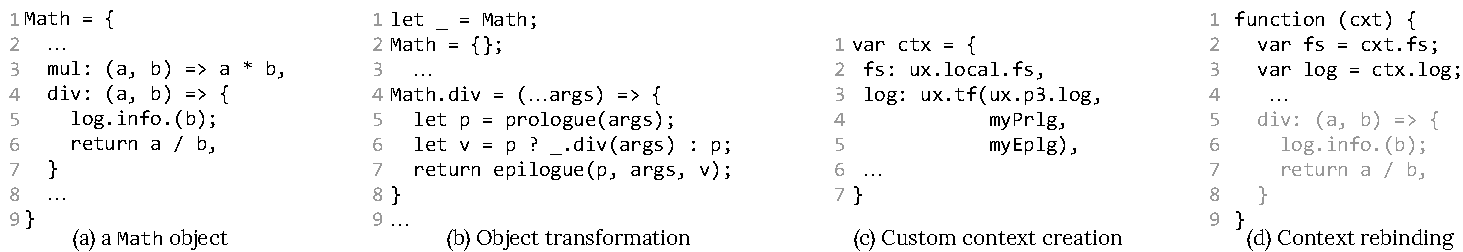
\includegraphics[width=0.99\textwidth]{./figs/lya_ex.pdf}
\vspace{-2mm}
\caption{
  \textbf{Example transformations.}
   Applying runtime transformations (b) and context rebinding (c, d) on a simple \ttt{Math} object~\cf{impl}.
}
\label{fig:tx2}
\vspace{-2mm}
\end{figure*}


At a very high level, loading a fresh module with \ttt{require("foo");} corresponds to the following five stages:

\begin{enumerate}
% \def\labelenumi{\arabic{enumi}.}
\item Resolution: identify the file to which the module specified corresponds, and locate it in the filesystem.
\item Loading: depending on the file type, use the corresponding loader (\eg V8 compiler for \ttt{js}, \ttt{JSON.parse} for \ttt{json} \etc).
\item Wrapping: wrap the module so that module-globals get encapsulated and Node.js globals (\eg \ttt{require}) get resolved.
\item Evaluation: evaluate the wrapped module in the current context, so that global names and top-level objects get resolved correctly.
\item Caching: add the module to a handful of module-related cache structures, for purposes of consistency and performance.
\end{enumerate}

% The resolution algorithm is somewhat convoluted, because it depends on several different facts (including the type of the file requested, whether it is a globally installed, whether it is a directory \etc).
% It does not require any \sys support beyond copying the directory that contains the source code of the all the modules onto the remote host.
\sys interposes on all of these steps to facilitate transformations.
Wrapping (3) and evaluation (4) are particularly interesting, because they allow \sys to interpose at the module boundary during runtime.
Before a module's code is evaluated, the Node.js module loader wraps the module so that
  (i) it keeps top-level variables (defined with \ttt{var}, \ttt{const} or \ttt{let}) scoped to the module rather than the global object; and
  (ii) it provides some global-looking variables that are actually specific to the module, such as the \ttt{module} and \ttt{exports} objects that the implementor can use to export values from the module and convenience variables---such as \ttt{\_\_filename} and \ttt{\_\_dirname}  containing the module's absolute filename and directory path, respectively.
True globals remaining are
  (i) the global objects as defined by the EcmaScript standard (\eg \ttt{Object}, \ttt{Function}, \ttt{Math}); and
  (ii) Node.js-specific globals (\eg \ttt{console}, \ttt{process}, \ttt{timer}).
These globals require further interposition.

% \begin{lstlisting}[language=js,mathescape,upquote=true]
% // Node.js will wrap a module with a function,
% // so as to bring certain names into scope
% // before compiling/evaluating code.
% let wrapped = "function (" +
%         "exports, require, module, " +
%         "__filename, __dirname, CTX) {" +
%     "let Math = CTX.Math" +
%     "let console = CTX.console" +
%     //...[more definitions]
%     moduleSource +
%   "});"
% \end{lstlisting}


\sys hooks into the wrapper function (the last variable in the function definition, \ttt{CTX}).
This trivial source-to-source transformation re-defines global variables as module-locals and initializes them with \sys-augmented values.
For example, \ttt{console} in the context of the module will be an \sys-created object that allows \sys to interpose on it.
Evaluation of the module passes an additional value to this function, which is the modified context.
As a result, any changes to the top-level objects and any global variables are accessible from the within the module.

% \begin{lstlisting}[language=js,mathescape,upquote=true]
% //Input: module ID e.g., absolute filepath
% let load = function (ID) {
%   if (cache[ID]) {
%      return cache[ID];
%   }
%   let m = {
%     exports: {}, id: ID, dir: path.resolve(ID)
%   };
%   let cm = v8.compile(wrapped);
%   let ii = iris.getImplicit(ID);
%   let c = iris.freshContext(ii);
%   cm(m.exports, this.require, m, ID, m.dir, c);
%   let ei = iris.getExplicit(ID);
%   m.exports = iris.wrap(m.exports, [ei] );
%   cache[ID] = m;
%   return m.exports;
% }
% \end{lstlisting}

The \ttt{load} method in the \ttt{Module} module combines evaluation (line 10) and caching (line 14) of the wrapped module.
After evaluation, invoking the compiled function generates the value that is assigned to \ttt{module.exports} from within the module (line 12).
\sys passes a freshly constructed context at that invocation, modified according to the implicit segment of the (PIC??) corresponding to the module being loaded.
Before returning the value of \ttt{module.exports}, \sys transforms it according to the explicit segment of the (PIC??) corresponding to the module being loaded.
Finally, the results of the entire process are placed into the module cache for later use.

\subsection{Limitations}

% FIXME: Talk about the inability to 
A limitation of our implementation is that it cannot analyze the library importing \sys---usually, the top-level program entry-point equivalent to \ttt{main}.
This is because \sys cannot transform the context of that file
As a result, \sys as-is cannot be applied to, say, to analyze single-file programs---a common pattern in scripting languages often used for quick-and-dirty tasks.
The simplest workaround here is to create an auxiliary file that imports \sys, and then import the single-file script (which, in most scripting languages would invoke it).



\section{Evaluation and Experience}
\label{eval}

\sys's  development achieves goals~\goal{1--3}~\sx{goals}, demonstrating that it is indeed feasible to construct a framework that operates at the level of modules, 
does not force developers to learn a new language, and that it can be implemented as a library around an existing runtime.
Despite the fact that it operates at coarser granularity, as shown earlier~\sx{impl} \sys can express analyses that generate results useful in several practical scenarios.

In this section, we are interested in zooming into \sys's performance characteristics~\goal{4}.
At a high level, we are interested in three questions:
(i) the overheads of the \sys's underlying building blocks;
(ii) the overhead of different analysis on real libraries and how this compares with production dynamic analysis frameworks; and
(iii) evaluation of \sys's behavior using our analyses on realistic, multi-library applications.
% For the first question, we use  synthetic micro-benchmarks that built to stress key elements of the system and confirm it works correctly~\sx{micro}.
% For the second question, we use real libraries and compare them with an analysis written in Jalangi~\sx{meso}.
% For the third question, we use a combination of real applications~\sx{macro}.

Several takeaways are worth highlighting.
\fixme{TODO after we have the results.}

Experiments were run on a moderate server with 4GB of memory and 2 Intel Core2 Duo E8600 CPUs clocked at 3.33GHz.
In terms of software, we used Docker version 18.09.7 running \fixme{a minimal Ubuntu XXX version}, Jalangi \fixme{vXXX}, Node.js v8.9.4 (bundled with V8 v6.1.534.50, LibUV v1.15.0, and npm v6.4.1), all atop a Debian Linux with kernel v4.4.0-134.
We run our software experiments within a Docker container to simplify the setup of the Jalangi framework.

\subsection{Micro-benchmarks}
\label{micro}

\sys's micro-benchmark suite was designed with two goals in mind.

The first goal was to test key properties of each analysis and confirm it outputs the expected results.
For example, to better understand performance diagnosis policy and confirm it works correctly, we craft a library that contains four other libraries with pre-defined bottlenecks.
The library can perform one of three operations, depending on its current state:
  (i) invoke a call to a module it imports,
  (ii) busy-wait, or
  (iii) respond to calls by returning a value.

The second goal was to identify understand \sys bottlenecks in a controlled environment, 
Both of these goals would have been difficult to achieve outside a synthetic environment, as we do not fully understand applications we haven't written ourselves.

\begin{table}[t]
\center
\footnotesize
\setlength\tabcolsep{3pt}
\caption{
  \footnotesize{
    \textbf{Synthetic Micro-benchmarks}.
		Applying the four analyses on a series of synthetic micro-benchmarks, created to stress different features.
  }
}
\begin{tabular*}{\columnwidth}{l @{\extracolsep{\fill}} ll lll}
\toprule
              &   Base    &  SA     & PD       &   TIC    &   LSR     \\
\midrule
something1    &           &  0.70   &    3.43  &   3.46   &   3.26    \\
something2    &           &  1.31   &    4.81  &   4.55   &   4.63    \\
something3    &           &  5.95   &    4.78  &   4.25   &   4.85    \\
something4    &           &  18.29  &   11.20  &   10.24  &   9.54    \\
something5    &           &  24214  &   24721  &   24574  &   24502   \\
\bottomrule
\end{tabular*}
\label{tab:synthetic}
\vspace{-5mm}
\end{table}

\begin{table}[t]
\center
\footnotesize
\setlength\tabcolsep{3pt}
\caption{
  \footnotesize{
    \textbf{Applying \sys to single-library programs}.
		\fixme{Execution time of four test suites against }
  }
}
\begin{tabular*}{\columnwidth}{l @{\extracolsep{\fill}} ll lll}
\toprule
                    & Base   &  SA   & PD     &   TIC   & LSR     \\
\midrule
Classnames~\cite{}  &  2.72  & 6.62  &  6.61  &  6.10   & 5.94    \\
Debug~\cite{}       & 31.39  & 33.54 &  33.94 &  33.96  & 33.04   \\
% Minimist\\
~~~-t1              & 31.46  & 60.13 &  60.00 &  56.62  & 56.72   \\
~~~-t2              & 19.17  & 59.77 &  60.75 &  57.15  & 57.79   \\
~~~-t3              & 21.64  & 205.2 &  205.53&  132.25 & 137.84  \\
~~~-t4              & 20.69  & 59.70 &  60.75 &  59.92  & 56.60   \\
~~~-t5              & 20.49  & 70.48 &  72.20 &  64.71  & 66.03   \\
Moment~\cite{}      & 31.73  & 48.04 &  49.23 &  44.95  & 46.12   \\
yargs~\cite{}       & 13.42  & 13.00 &  14.41 &  13.47  & 13.48   \\
\bottomrule
\end{tabular*}
\label{tab:meso}
\vspace{-5mm}
\end{table}


Table~\ref{} depicts the results of the four analysis applied to these benchmarks.
We decided to report all combinations of analyses and benchmarks, but in practice not all are useful---\eg some modules do not feature interesting access or performance patterns.
Currently, these benchmarks return the results we expect, but they did help with the identification of problems such as 
These be
Load is visible at the application level (left), but the lack of detail does not help determine which modules must be scaled out.
Module-level data, collected by \sys' coordinator (right), reveal that \ttt{m3} receives the majority of the load.

To understand the costs of proxy interposition, we measure the time to access deeply-nested properties of two versions of an object:
  unmodified and proxy-wrapped.
Paths to the properties (\eg \ttt{a.b.c.$\ldots$}) are random but generated prior to running the experiment.
We construct 500MB-sized objects, each with a fanout of 8 fields nested for 12 levels.
The proxy-wrapped version introduces interposition at every level.
Traversing one million 12-edge paths (\ie root to leaves) averages 167.2ms and 595.7ms for the unmodified and proxy-wrapped versions, respectively.

We emphasize that this is an artificially constructed benchmark stressing worst-case overheads nowhere near an normal execution:
  for comparison, the transformation of these objects itself took nearly 16 seconds ($10^3\times$ more than what we experienced with real modules).
The takeaway is that \sys-inherent overheads due to interposition are unlikely to be the bottleneck of an analysis.

\subsection{Single-module Benchmarks}
\label{meso}

\begin{figure*}[t]
  \centering
   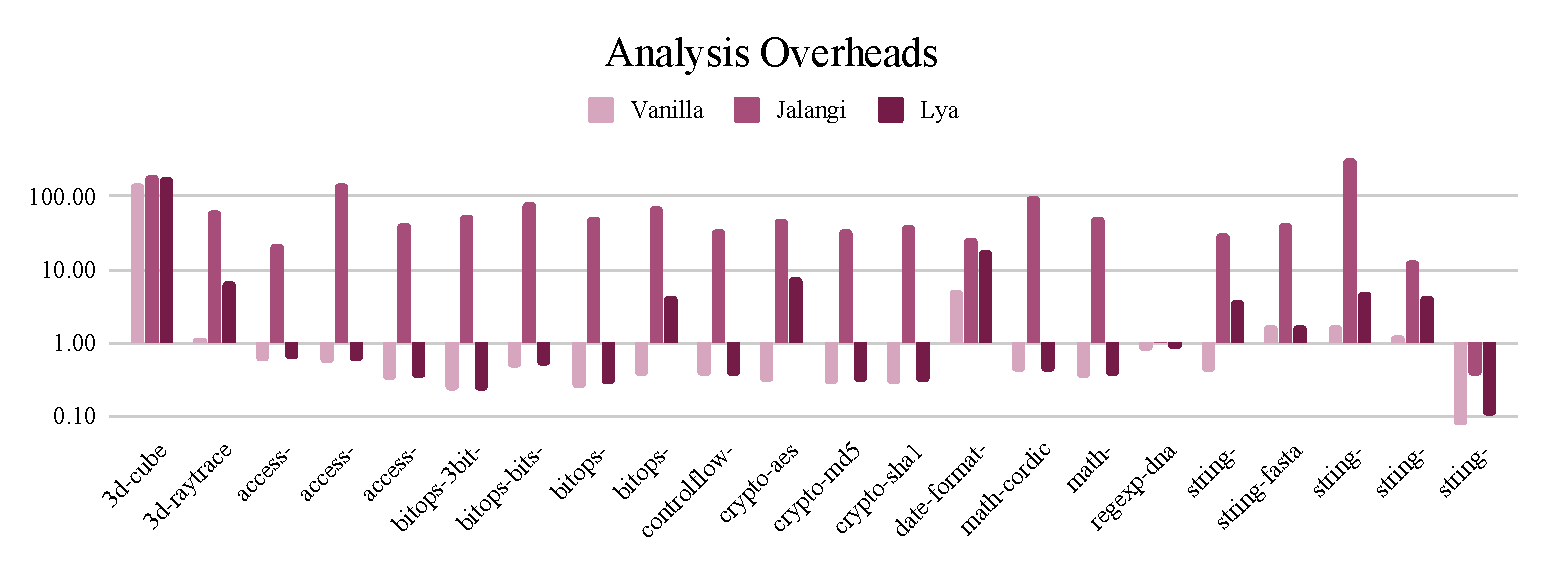
\includegraphics[width=0.95\textwidth]{./figs/meso.pdf}
  \caption{
    \textbf{Analysis overheads.}
    The plot compares a series of modules from single-library programs taken from Jalangi between three setups:
		(i) Vanilla JavaScript, (ii) global-use analysis using Jalangi, (iii) global-use analysis using \sys.
    Global-use analysis is a relatively simple analysis that tracks accesses of global variables in the program~\cf{meso}.
  }
  \label{fig:meso}
  \vspace{-3mm}
\end{figure*}


\subsection{End-to-End Benchmarks}
\label{macro}

\begin{table}[t]
\center
\footnotesize
\setlength\tabcolsep{3pt}
\caption{
  \footnotesize{
    \textbf{Applying \sys to three large applications}.
		\fixme{Highlight some things}
  }
}
\begin{tabular*}{\columnwidth}{l @{\extracolsep{\fill}} lll}
\toprule
                    & Koa    & Moeda   &  Terminalizer \\
\midrule
 Size (KB)          & 41M    &  29M    &   262M        \\
 LoC                & 127K   &  79K    &   39K         \\
 Top-level modules  &  24    &  7      &    33         \\
 Total Modules      &  432   &  260    &    1084       \\
 Lya detects:       &  1507  &   729   &     2355      \\
 Baseline           &  xx    &         &               \\
 A1 (TF)            &        &         &               \\
 A3 (HF)            &        &         &               \\
 A8 (Types)         &        &         &               \\     
\bottomrule
\end{tabular*}
\label{tab:macro}
\vspace{-5mm}
\end{table}



Highly popular applications---for example, Koa.js and Terminalizer have 28.3K and 8.7K stars stars on GitHub, respectively.
Applying \sys to these applications generates much larger analayses
For example, the performance diagnosis analysis hooks reports timing characteristics for 

The difference between the modules detected statically (by running \ttt{npm ls}) and the ones observed by \sys is due to a few different reasons.
One is that an analysis does not report accesses if a 
\sys analyzes modules that are part of the standard library too (some of which have themselves internal dependencies), which are not shown by \ttt{npm}.
Our post-processing counts by module name (\ie squashes duplicate reports by 
This can affect the results of multiple imports with the same name at different parts of the tree that would indeed correspond to different.
For example, importing two different versions of a library at two different parts of the dependency tree will result in to two different with the same name.
It also squashes cache entries that correspond to one module imported by multiple modules, which would create separate entries in \sys's augmented cache, but would result in a single count for Tab.~\ref{macro} (for \sys's treatment of the module cache, see~\S\ref{cache}).
Confirming that \sys performs correctly under these scenarios is one part of the motivation behind the synthetic micro-benchmarks shown earlier~\sx{micro}.


\section{Discussion}
\label{diss}


Library dialysis, as implemented in \sys, depends on a few features available in the programming language.
In this section we describe how to develop the same solution on other environments.
In the second part of this section, we reflect on some of the current limitations of the system.

\subsection{Applying to Other Environments}
\label{reqs}

\begin{table*}[t]
\center
\footnotesize
\setlength\tabcolsep{3pt}
\caption{
  \footnotesize{
    \textbf{Language features used and their availability in other languages}.
    Broadly, the requirements of module dialysis can be broken down into to five elementary requirements.
  }
}
\begin{tabular*}{\textwidth}{l @{\extracolsep{\fill}} lll ll}
\toprule
             &  Instrument \ttiny{import}s  & Traverse objects      & Wrap values         & (Weak) Maps       & Shadow variables      \\
\midrule
Lua          &                              &                       &                     &                   &                       \\
JavaScript   &                              &                       &                     &                   &                       \\
Python       &                              &                       &                     &                   &                       \\
Ruby         &                              &                       &                     &                   &                       \\
Haskell      &                              &                       &                     &                   &                       \\
OCaml        &                              &                       &                     &                   &                       \\
Rust         &                              &                       &                     &                   &                       \\
Java         &                              &                       &                     &                   &                       \\
\bottomrule
\end{tabular*}
\label{tab:compat}
\vspace{-5mm}
\end{table*}

The techniques presented in this paper are applicable to any programming language.
We chose the JavaScript ecosystem to evaluate the feasibility of our approach, primarily because
  (i) it boasts the largest collection of libraries (and number of problems)~\cite{modulecounts} and
	(ii) we had prior experience by writing two systems that make extensive use of dynamic analysis---more sophisticated versions of analyses \fixme{XX} and \fixme{XX}.
In this section, we discuss the requirements for building \sys over other runtime environments.
% FIXME: All these features have to have been discussed earlier

By operating on library boundaries, program dialysis makes use of five key features available in a programming language~\tb{compat}.
All major programming languages can support these five features in a variety of ways, as described below.

First, \sys replaces the implementation of the import statement (\eg \ttt{require}).
% This feature is important for compatibility reasons---otherwise developers would have to replace all import statements in their applications.
If this statement is a function (\eg JavaScript, Scheme, Racket \etc) then replacement can be easily achieved by replacing its definition.
If this statement is a special non-function keyword such as \ttt{import}, this can be achieved by a rewriting rule that replaces import with a special function;
% This is simplified by the fact that the import syntax is trivial.

\sys also needs the ability to interpose on values and transform their components.
This is relatively easy in languages that provide meta-programming capabilities.
Dynamic programming languages offer runtime reflection and conveniently expose object accesses as (over-loadable) functions---\eg \ttt{Proxy} objects in JavaScript, metatables in Lua, metaclasses in Python, and direct-accessor meta-programming Ruby.
Compiled languages such as Haskell, OCaml, and Rust would apply transformations with static metaprogramming facilities, traversing and transforming objects at compile time.
Examples include templates and macro expansions such as Haskell's Template Haskell and Rust's macro system.
And some languages, such as Haskell, Java, and Julia, provide both static and dynamic reflection capabilities, allowing considerable freedom in the choice of implementation.
% Fifth, \sys makes extensive use of interposition which is also available in different programming languages.
% Static programming languages provide different types of support for 

\sys makes extensive use of weak maps to support to check for object equality.
Examples of uses include checking for cycles during object traversal and checking whether an object has already been wrapped.
Hash tables that are indexed by reference are supported in virtually all programming languages.
An additional feature useful in garbage-collected languages would be for these (copies of) references to not affect the reclamation of original objects.
Languages either support the ability to create such a weak reference from a normal reference (\eg Python's weak references), or provide structures that automatically hold weak versions of these references (\eg JavaScript's Weak Map).

Finally, \sys makes extensive use of variable shadowing to hide access to the original, unmodified versions of values.
This is a feature that is universally available in programming languages;\footnote{
  A notable exception is the language CoffeeScript. %, which can mimic the same feature using function scope.
}
Deferences in scoping rules---\ie what the shadowed variable ends up referring to upon execution---do not affect the usefulness of this feature, although we have found lexical scoping easier than dynamic scoping.

To conclude, all major languages provide enough facilities to support the dialysis---albeit with a different level of convenience.
Dynamic languages have features---\eg name (re-)binding, value introspection, dynamic code evaluation, and access interposition---that enable runtime transformations.
Runtime transformations conveniently unify module identification with interposition:
  a single function or function-like operator locates a module, interprets it, and applies transformations before exposing its interface in the caller context.
Compiled languages such as Haskell, OCaml, and Rust apply transformations using compile-time metaprogramming facilities.
Compile time transformations alleviate much of the runtime overhead of transformations, improving program startup times;
  and type checking could further aid developers by issuing warnings of incompatible privilege settings.


\subsection{When to Use Dialysis}
\label{principles}
Dynamic analysis is a general analysis technique that discovering facts about programs.
While full-fledged dynamic analysis can provide full visibility into , it may result in higher performance overheads and developer effort.
Dialysis can be thought as a coarser version of analysis stemming from the natural boundaries of libraries, a level of granularity that is just right for certain domains.
Which are these cases exactly?

The first class of  
It is really a quick-and-dirty 
As it quickly isolates homegrown code from standard libraries and third-party code, it is a help pin-point to 
Its availability as a global module makes this trivial.
% This is a particularly good match for dynamic programming languages that are already geared towards quick prototyping.

The second is when the goal is to understand the behavior of third-party code.
Dialysis plugs monitors all around a library, and in clearly delineated abstraction boundaries within that library where the signal-to-noise ratio is naturally expected to be high.
Dialysis deconstructs programs only at the library boundaries, at a granularity well-suited for several tasks.
Examples include the 
N-version programming ---all of which would require a custom tool.
By viewing the program's surrounding environment as libraries---which is the case in all high-level programming languages---dialysis can expand its coverage to the operating system, file system, network and other ``ambient'' services.

Dialysis is \emph{not appropriate} for monolithic programs or ones written in low-level languages such as C.
These limitations is due to several reasons.
First, C programs do not feature clear, ``impenetrable'' boundaries like the ones available in memory- and type-safe languages.
An important feature of the wrapping techniques presented in this paper is that they can ---\ie the full observable behavior around a library.
Unfortunately, this is not true in C where a library can forge a pointer and access arbitrary locations in its the program's address space.
A related problem is the inability to traverse and wrap objects, due to lack of bounds.
It is unclear how to wrap values without any kind of size information.\footnote{
  Recent advances show promise: C-Strider~\cite{saur2016cstrider} and ptrSplit~\cite{ptrsplit:17} provide type-aware heap traversal for C programs.
}
% Finally, C is missing direct direct equivalents to \sys's requirements~\sx{reqs}

That said, it is possible to apply dialysis in C programs that have first gone through a process of decomposition or component sanboxing---as is the case in compartmentalization, program slicing, and related areas.
Additionally, many libraries in high-level programming languages today simply wrap C programs either directly or through a foreign-function interface.
Dialysis can be used with these libraries, as it plugs into the abstractions provided by the high-level, wrapper interface.

\section{Related Work}
\label{rw}

In this section, we compare \sys to previously proposed systems in several categories.
For a comparison between dialysis and dynamic analysis, we refer the reader to the previous section~\sx{principles}.

% \heading{Dynamic Analysis Systems}
There are several dynamic analysis frameworks for JavaScript~\cite{javascript1, javascript2, javascript3, mugshot, jalangi}.
The two most popular, Jalangi~\cite{jalangi} and Mugshot~\cite{mugshot}, are fine-grained code-level instrumentation tools.
On top of analysis, their heavy instrumentation is powerful enough to record and replay entire program executions.
This power comes at a significant performance cost---typically 2--3 order-of-magnitude slowdown---as they need to virtualize the entire execution environment:
  source-code-level rewriting every expression corresponding to a profiling event in the original program needs is resolves to a profiling function call.
They are also not embeddable in existing applications in a runtime-agnostic manner.
These features are contrary to \sys, which leverages fairly basic programming-language techniques such as variable shadowing and context transformation during library loading to insert analysis hooks completely transparently to the runtime environment.

NodeProf~\cite{javascript3} is a fine-grained dynamic analysis implemented using Truffle~\cite{} and running on top of Graal.js [28], a Node.js-compatible runtime.
NodeProf stands at a different point in the analysis design space---more powerful than \sys, but with significantly more effort.
It statically instruments the program's AST (rather than the code), making it easier to maintain compared to source changes but assuming some knowledge of the Graal and Truffle APIs and requiring recompilation of the Java hooks.
Different from \sys, it leverages AST extraction and manipulation to build, which is not available in many languages and may be limit by dynamic features such as reflection and JITing.
Nevertheless, NodeProf's approach shares similarities with \sys, including decoupling from the source code, overheads lower than code instrumentation, and can on/off toggling during execution.
%FIXME: Lya is also limited (i) by dynamic features such as reflection, because they're gonna hit the wrapper and (ii) the equality and other primitive operators

Aran~\cite{javascript1}, an implementation sketch of proxy-based analysis, leverages JavaScript's \ttt{with} primitive to wrap custom contexts.
\sys works at the module boundaries (at a potentially coarser granularity) without any special language constructs.

JSConTest2~\cite{javascript2} is a dynamic \emph{access} analysis framework, similar to \sys's analysis \fixme{A2}, build around proxies.
It allows users to write access control contracts, policies that execute at runtime.
It illustrates the need for a general-purpose framework such as \sys, as many of JSConTest2's access permission contracts are 
Our evaluation shows that this analysis (and others) can be implemented on top of \sys with significantly less effort.


\heading{Dynamic Analysis for WebAssembly}
Related to JavaScript is WebAssembly, a standardized subset of JavaScript target, designed to serve as a compilation target.
The first dynamic analysis framework for WebAssembly, Wasabi~\cite{wasabi}, shares some of the same goals with \sys---\eg lowering the effort required to write analyses, and providing hooks for observation rather than manipulation.
Wasabi is also programmable in JavaScript (which, however, is not its target language), a similarity to \sys that is mostly accidental:
  Wasabi needs to be provide a high-level analysis scripting interface and chose JavaScript;
  whereas our explicit goal is to write analysis in the same language as the program~\sx{goals}---that is, dialysis implemented for Python would be using Python abstractions.
Contrary to \sys, Wasabi instruments binaries statically, \ie ahead-of-time, and aims on heavyweight instrumentation.



\heading{Dynamic Instrumentation}
Dialysis is related to dynamic instrumentation frameworks~\cite{pin, valgrind} that wrap incrementally parts of the program to extract information.
Pin~\cite{pin} and Valgrind~\cite{valgrind} translate basic blocks of the program just before their execution;
  \sys starts by wrapping a library during import, adding a small overhead on its loading time.
This overhead is only a small fraction of the time required to locate and load the module from disk.
However, these systems operate at a much lower level (binary) than \sys, and are not available to high-level runtime environments as a pluggable library.

DiSL~\cite{disl} and RoadRunner~\cite{roadrunner} are systems for instrumenting JVM byte code.
These too work at a lower level than \sys, 

\heading{Program Transformations}
% Add our work
Module dialysis builds on aspect-oriented programming (AOP), a programming model where program points map to actions taken at these points~\cite{aop}.
Both approaches lower complexity by mapping multiple points across the program to the same actions, but dialysis does not alter the program's control flow.
Moreover, AOP works on languages that were already designed to support it, whereas module dialysis is explicitly designed to bolt onto existing languages.

More generally AOP is related to metaobjects~\cite{metaobject}, objects that manipulate object structure, and which enable a program to access to its own internal structure, including rewriting itself as it executes.
While \sys makes extensive use of metaobjects to traverse, understand, wrap, and rewrite interfaces, it shields developers from building the required metaobject infrastructure.
% self element

\heading{Fracture and Recombination}
Dialysis draws inspiration directly from program fracture and recombination (PFR)~\cite{fracture1, fracture3}, a line of work less tied to program analysis and more towards program synthesis and automated patch generation.
PFR breaks up multiple programs into many components with the goal of exchanging functionality between donor-donee pairs of programs.
Contrary to PFR, dialysis operates on single programs, avoids breaking semantics, and leverages the existence of components with (mostly) explicit boundaries in the guise of libraries or modules.

\section{Conclusion}
\label{end}

Recent trends in software engineering have led to unprecedented levels of third-party code re-use.
Applications today routinely pull together hundreds of libraries, making their analysis difficult 

due to the very same abstraction and modularity principles that have benefited software engineering for decades.

security auditing and performance profiling---already challenging in monolithic applications---become extremely difficult in the presence of deeply-nested third-party code.

This paper introduces \emph{module dialysis}, an approach 
corser
approach towards coarse-grained
This is achieved using a set of programmatic \emph{transformations} parametrizable by optional \emph{distribution recipes}.
These operate at module boundaries during runtime to collect profiling information, detect bottlenecked components, and dynamically separate and coalesce parts of the application.

We want to emphasize that \sys is open source, available to experiment with more applications and analyses

% \section*{Acknowledgments}
% Martin
% \section*{Availability}

\bibliographystyle{plain}
\bibliography{bib}

\end{document}

%%  LocalWords:  endnotes includegraphics fread ptr nobj noindent
%%  LocalWords:  pdflatex acks
